\documentclass[sigplan,screen]{acmart}

\usepackage[utf8]{inputenc}
\usepackage{microtype}

\AtBeginDocument{%
  \providecommand\BibTeX{{%
    \normalfont B\kern-0.5em{\scshape i\kern-0.25em b}\kern-0.8em\TeX}}}

\setcopyright{acmcopyright}
\acmPrice{}
\acmDOI{10.1145/3426431.3428656}
\acmYear{2020}
\copyrightyear{2020}
\acmSubmissionID{splashe20main-id5-p}
\acmISBN{978-1-4503-8180-2/20/11}
\acmConference[SPLASH-E '20]{Proceedings of the 2020 ACM SIGPLAN SPLASH-E Symposium}{November 20, 2020}{Virtual, USA}
\acmBooktitle{Proceedings of the 2020 ACM SIGPLAN SPLASH-E Symposium (SPLASH-E '20), November 20, 2020, Virtual, USA}



\begin{document}
\title[Objective Typography]{CSS Instruction Enhanced by Objective Typography}

\author{Karl Stolley}
\email{kstolley@iit.edu}
\orcid{1234-5678-9012}
\affiliation{
  \institution{Illinois Institute of Technology}
  \streetaddress{Institution Street Address}
  \city{Chicago}
  \state{IL}
  \country{USA}
  \postcode{60616}}

\begin{abstract}
This course experience report details an approach for teaching Cascading Style Sheets (CSS) constrained by the rules of objective typography. The approach condenses CSS to a human-scaled but representative subset of fewer than a dozen properties, which students then apply to a fundamental problem of visual communication: setting text that is accessible and readable across the range of screens on web-enabled devices. Students discover how to determine rule-governed values and ratios according to typographic principles, which are in turn applied and modified in a predictable, mathematically harmonious way across an entire website via its style sheet. Students learn how to verify visual results under particular viewing conditions before refactoring their work to accessibly engineer the web for diverse groups of human users. Experiential evidence suggests that these techniques transfer to other aspects of CSS, but formal study is needed.
\end{abstract}

\begin{CCSXML}
<ccs2012>
<concept>
  <concept_id>10003456.10003457.10003527.10003531.10003535</concept_id>
  <concept_desc>Social and professional topics~Information technology education</concept_desc>
  <concept_significance>500</concept_significance>
</concept>
<concept>
  <concept_id>10003456.10003457.10003527.10003528</concept_id>
  <concept_desc>Social and professional topics~Computational thinking</concept_desc>
  <concept_significance>300</concept_significance>
</concept>
</ccs2012>
\end{CCSXML}

\ccsdesc[500]{Social and professional topics~Information technology education}
\ccsdesc[300]{Social and professional topics~Computational thinking}

\keywords{Cascading Style Sheets, typography, web design, curriculum}


\maketitle

\section{Introduction}

At least two factors make CSS a challenging language to teach. First, CSS bears little resemblance to other languages in the web curriculum or in the curriculums of computer science and information technology generally. Even comparing languages only in the web curriculum, HTML can trace its ancestry to SGML and its contemporaries to XML. JavaScript has a complicated history but shares the features of many prototyped, procedural languages. By contrast, CSS’s closest relative is an obscure one: Simple Tree Transformation Sheets (STTS)\cite{w3c:briefhistory}, which used the selector-declaration syntax found in CSS. CSS's outlier status means that knowledge of other languages has limited transfer to CSS.

Second, CSS is a challenge to teach because the language continues to grow. Since the original CSS specification was published in late 1996, the CSS language has expanded considerably in capability as well as complexity: the 53 properties in the CSS 1 specification more than doubled to 115 in CSS 2.1/2.2. The modules that comprise CSS3 included some 363 properties \cite{jom:css}. As of late 2020, the World Wide Web Consortium (W3C) estimates that CSS contains or is proposed to contain 533 distinct properties, spread across 145 different technical reports and editors' drafts \cite{w3c:iop}. At its most basic, CSS works by targeting and styling specific structures found in HTML documents. Because each CSS property has a very specific purpose (specifying text and background colors; italicizing or bolding text, for basic examples), CSS properties are not generalizable or easily used to suit other purposes. That stands in contrast to the core methods and functions of most other languages. Instruction in CSS can therefore devolve into trying to cover a growing list of properties.

 Students also face their own challenges learning CSS. As the language has grown, overwhelmed students often skip the fundamentals in favor of searching for tutorials that describe complicated visual effects and gimmicks, such as parallax scrolling, which inevitably lead to a lot of cut-and-paste code and little transferable learning.

The approach to CSS instruction constrained by typographic principles addresses and attempts to solve the following problems students routinely face learning CSS:


\begin{itemize}
  \item \textbf{Where to start?} CSS can specify many visual qualities,  in just about any order. CSS neither enforces an order nor establishes any given properties as necessary, in contrast to the precise requirements of HTML.
  \item \textbf{What values to use?} And what units to express CSS values in? Left to their own devices, students pick values more or less out of thin air, or from other, inappropriate contexts: {\itshape Google Docs defaults to a text size of 11, so I’ll use 11 on this web page, too.}
  \item \textbf{When is it “finished”?} Compared to a set of style declarations in CSS, the content-completeness of an HTML document or the feature-completeness of a JavaScript function are more obviously verified, even by beginners.
\end{itemize}




\subsection{Instructional Context}
The approach to CSS instruction described here has been used several times over a period of four years in the first of a two-course sequence in introductory web-development. Both courses in the sequence are required of all undergraduate majors in an information technology and management program. The first course covers the syntax and semantics of standards-based HTML, CSS, and JavaScript, which the second course applies to web design problems anchored by theories of user-centered design and human-computer interaction.

The course typically enrolls between 30 and 40 students. Classroom instruction proceeds largely as demonstration-based, live-coded lectures. Students complete between five and ten smaller lab assignments, including one on objective typography and CSS. The bulk of student work is organized around three major projects. The first project is the semantic HTML foundation for a multi-page website. The second project adds CSS to that work, while students continue to refine and improve their HTML. The third and final project is a revision of the second project, based on multiple rounds of peer and instructor feedback, and requires students to include a JavaScript feature. A copy of the complete course syllabus is available on the web\cite{kas:fwd}.

Both courses in the sequence teach accessibility as a core web-engineering principle. That is expressed in part by the philosophy of progressive enhancement, which is reflected in the course projects. Progressive enhancement begins with a foundation of semantic HTML free from all presentational elements and attributes. The HTML is then styled by a design layer expressed in single site-wide CSS file. The HTML and CSS are then augmented by unobtrusive JavaScript that leverages event listeners to manipulate the browser’s Document Object Model (DOM) for interactivity and page enhancements not achievable by HTML or CSS alone.

The instructional approach to CSS described here emphasizes the first course’s focus on language features: although derived from visual design, typographic principles provide students with a thorough and human-scaled approach to CSS as a language, rather than a tangential engagement with a design aesthetic.

\subsection{Instructional Approach in Brief}

Introducing CSS constrained by typographic principles is intentionally deceptively simple. It restricts students to using fewer than a dozen CSS properties necessary to establish a typographic grid and a modular typographic scale. The grid establishes a repeating baseline for text to sit upon, while the modular scale provides a mathematically harmonious range of alternative type sizes anchored by a readable, accessible base font size.

\begin{figure}
  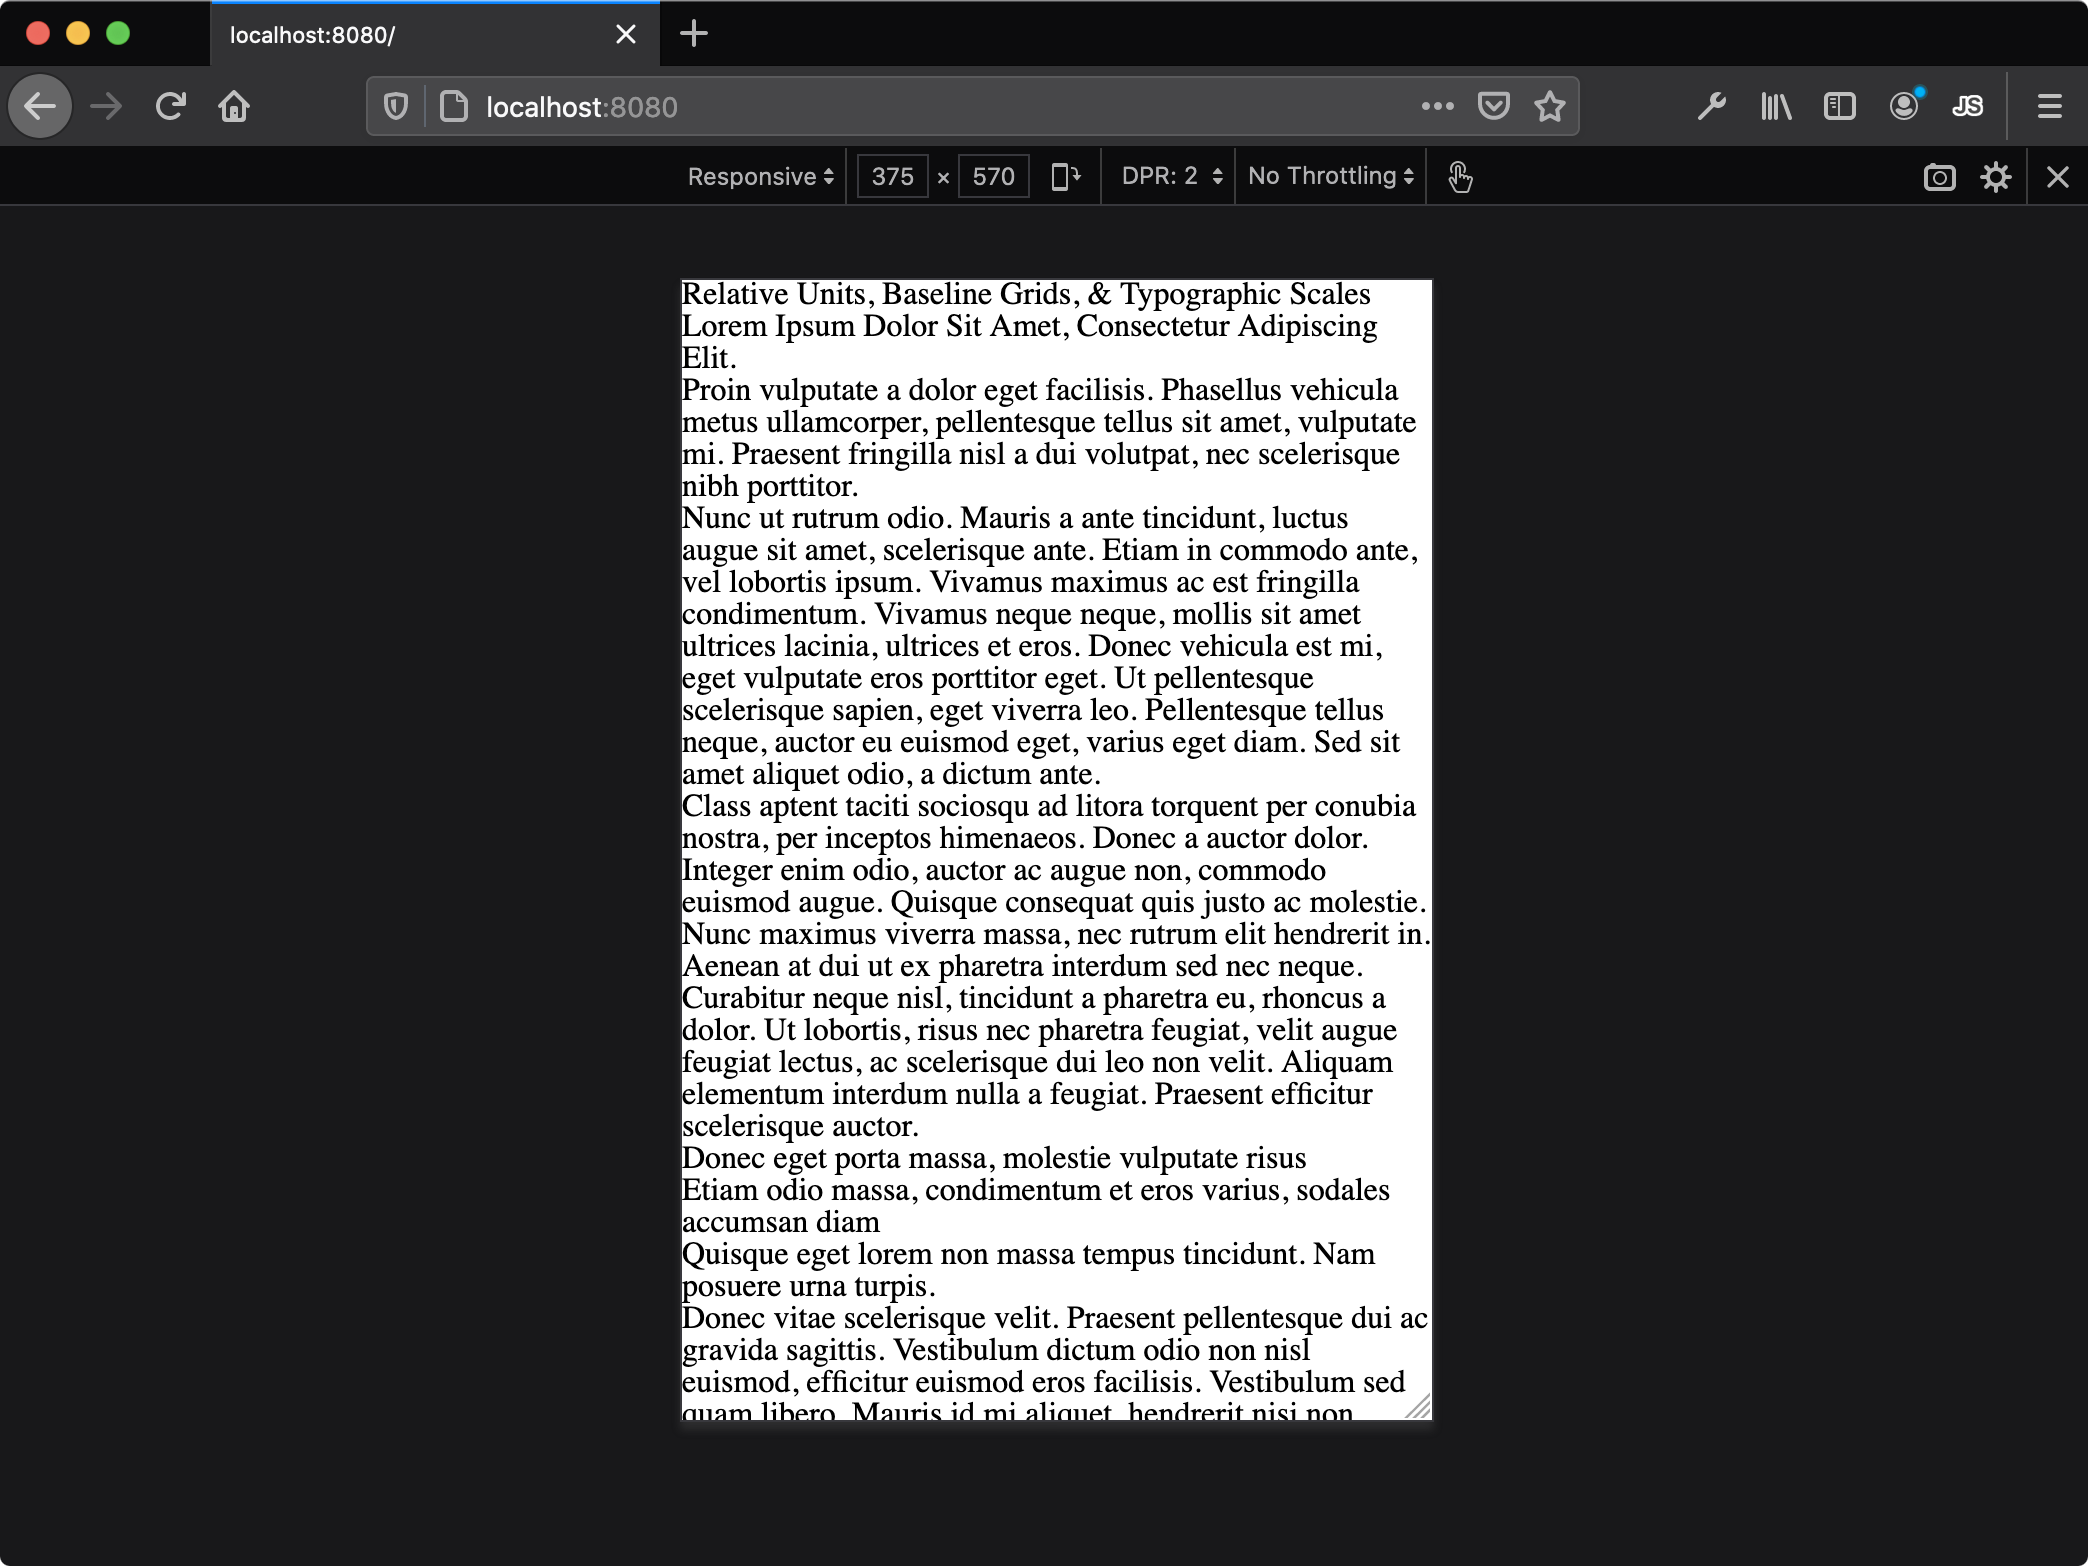
\includegraphics[width=\linewidth]{rdv}
  \caption{The responsive design view (RDV) in Mozilla Firefox.}
  \Description{A screenshot showing a page of HTML in a browser, with reset styles applied.}
  \label{fig:rdv}
\end{figure}

Students begin by working with the responsive design view (RDV) in a development browser such as Mozilla Firefox Developer Edition (Figure \ref{fig:rdv}). The RDV should be collapsed to a size that approximates the dimensions of a mobile phone. Students should be shown how and encouraged to make use of a lightweight local web server, such as the \verb|http-server| package written for Node.js \cite{npm:http}, so that they can learn as early as possible to view projects in progress over the local network on actual mobile and tablet devices, not just their own chosen development browser.

\section{Objective Typography Principles}

Typography represents among the most humanized aspects of visual communication. Graphic designer Ellen Lupton observes that “Words originated as gestures of the body. The first typefaces were modeled on the forms of calligraphy.” \cite[p.~13]{el:type}. The establishment of objective rules for the use of type--“the correct spaces between letters and words and the length and spacing of lines conducive to easy reading” \cite[p.~19]{mb:grid}--trace their origins to the at least the Industrial Revolution. They achieve fuller and more exacting description in the work of mid-twentieth-century European designers such as Josef Müller-Brockmann’s {\itshape Grid Systems in Graphic Design}, which specifically labeled the principles as constituting “objective typography” \cite[p.~7]{mb:grid}.

The basic rules of objective typography are echoed and refined across a number of contemporary book-length works that I have assigned in whole or as excerpts in web development classes: Ellen Lupton’s {\itshape Thinking with Type}, Robert Bringhurst’s {\itshape The Elements of Typographic Style}, and David Jury’s {\itshape About Face: Reviving the Rules of Typography} \cite{el:type,rb:style,dj:face}. An open-access book that has also been a student favorite is Matthew Butterick’s {\itshape Practical Typography} \cite{mb:pt}.

Objective typography requires the selection of a readable type size and setting a predictable baseline grid for the extent of a page. To build structure and make text more readable, a modular scale provides a mathematically harmonious set of values for setting display type (such as headlines and headings) and caption type (literal captions on figures as well as other small print). All running text as well as display and caption text rest uniformly on the page’s typographic grid lines, which also suggest values for offsetting blocks of text from one another in a predictable, mathematically harmonious way.

\section{Instructional Rationale and Method}

Applied to CSS instruction, objective typography offers a number of advantages:

\begin{itemize}
  \item It is rule- and principle-governed, which clarifies the objectives of both instruction and assessment
  \item It limits the scope of initial CSS instruction to just a handful of properties and techniques
  \item Its expression in CSS exposes students to numerous features of the language, especially inheritance, where a value set on one property affects the initial value or behavior of another property, even when set on another HTML element
  \item It introduces students to the process of translating and transposing external rules or visual plans from abstract concepts to concrete declarations in CSS
  \item It establishes a core set of values and units that can be carried over into advanced layout methods and grid-based design
\end{itemize}

Note that applying the fundamental principles of objective typography does not come close to fully exhausting the possibilities of CSS typography: the basic instructional approach excludes typographic flourishes and stylistic enhancements, especially font variants such as small caps, that can now be represented in stunning clarity on high-density displays.

For the purposes of learning this technique, students can be provided with a semantically structured HTML document from the instructor, or they can work from their own HTML, perhaps as part of a larger project. The HTML should use the viewport \verb|<meta>| element to set mobile devices to display at their native resolutions.

Because of the varying availability of typefaces on different operating systems, instructors should suggest a few web-available typefaces, such as from Google Fonts, for students to work with. Ideally, the candidate typefaces should have anatomical features that lend themselves to long-form reading: moderate stroke contrast, a large x-height, and pronounced ascenders and descenders. The typefaces in Figure \ref{fig:bvos} all exhibit those features.

Teaching CSS constrained by objective typography is a systematic process: after applying a reset stylesheet, which effectively strips away all default browser styles \cite{em:rc}, students work with a mobile-sized viewport to determine a reasonable size for the body copy, initially expressed in absolute, pixels units. From there, students experiment to find an appropriate leading (pron. {\itshape ledding}) to separate the lines of running text. That value is set on the CSS \verb|line-height| property, and becomes the fundamental base-line grid for the page. Block elements (headings, paragraphs, lists and list items) can then be offset from one another with additional vertical space, based on the fundamental \verb|line-height| value. Students then convert those absolute values into relative values for greater accessibility. Finally, students begin to open up the RDV to larger viewports and make targeted adjustments to their stylesheets, often using CSS media queries, to ensure an optimal text setting across a full range of device and viewport sizes.

\subsection{Sizing Body Type}

Selecting an appropriate size for body type is the most critical step in the process, because that size value determines all of the other values that follow. While keeping critical eyes on both the RDV emulator and the mobile phone, students can begin to experiment discovering a suitable base font-size for the page.

Students are surprised to learn that there isn’t a universal readable-size value: because the optical size of a typeface (that is, its visible letterforms) differs from its body size (the invisible boxes around letterforms), as shown in Figure \ref{fig:bvos}, there is no universal readable-size value--only certain likely ranges of sizes, which must be carefully adjusted based on the unique characteristics of a given typeface.

\begin{figure}
  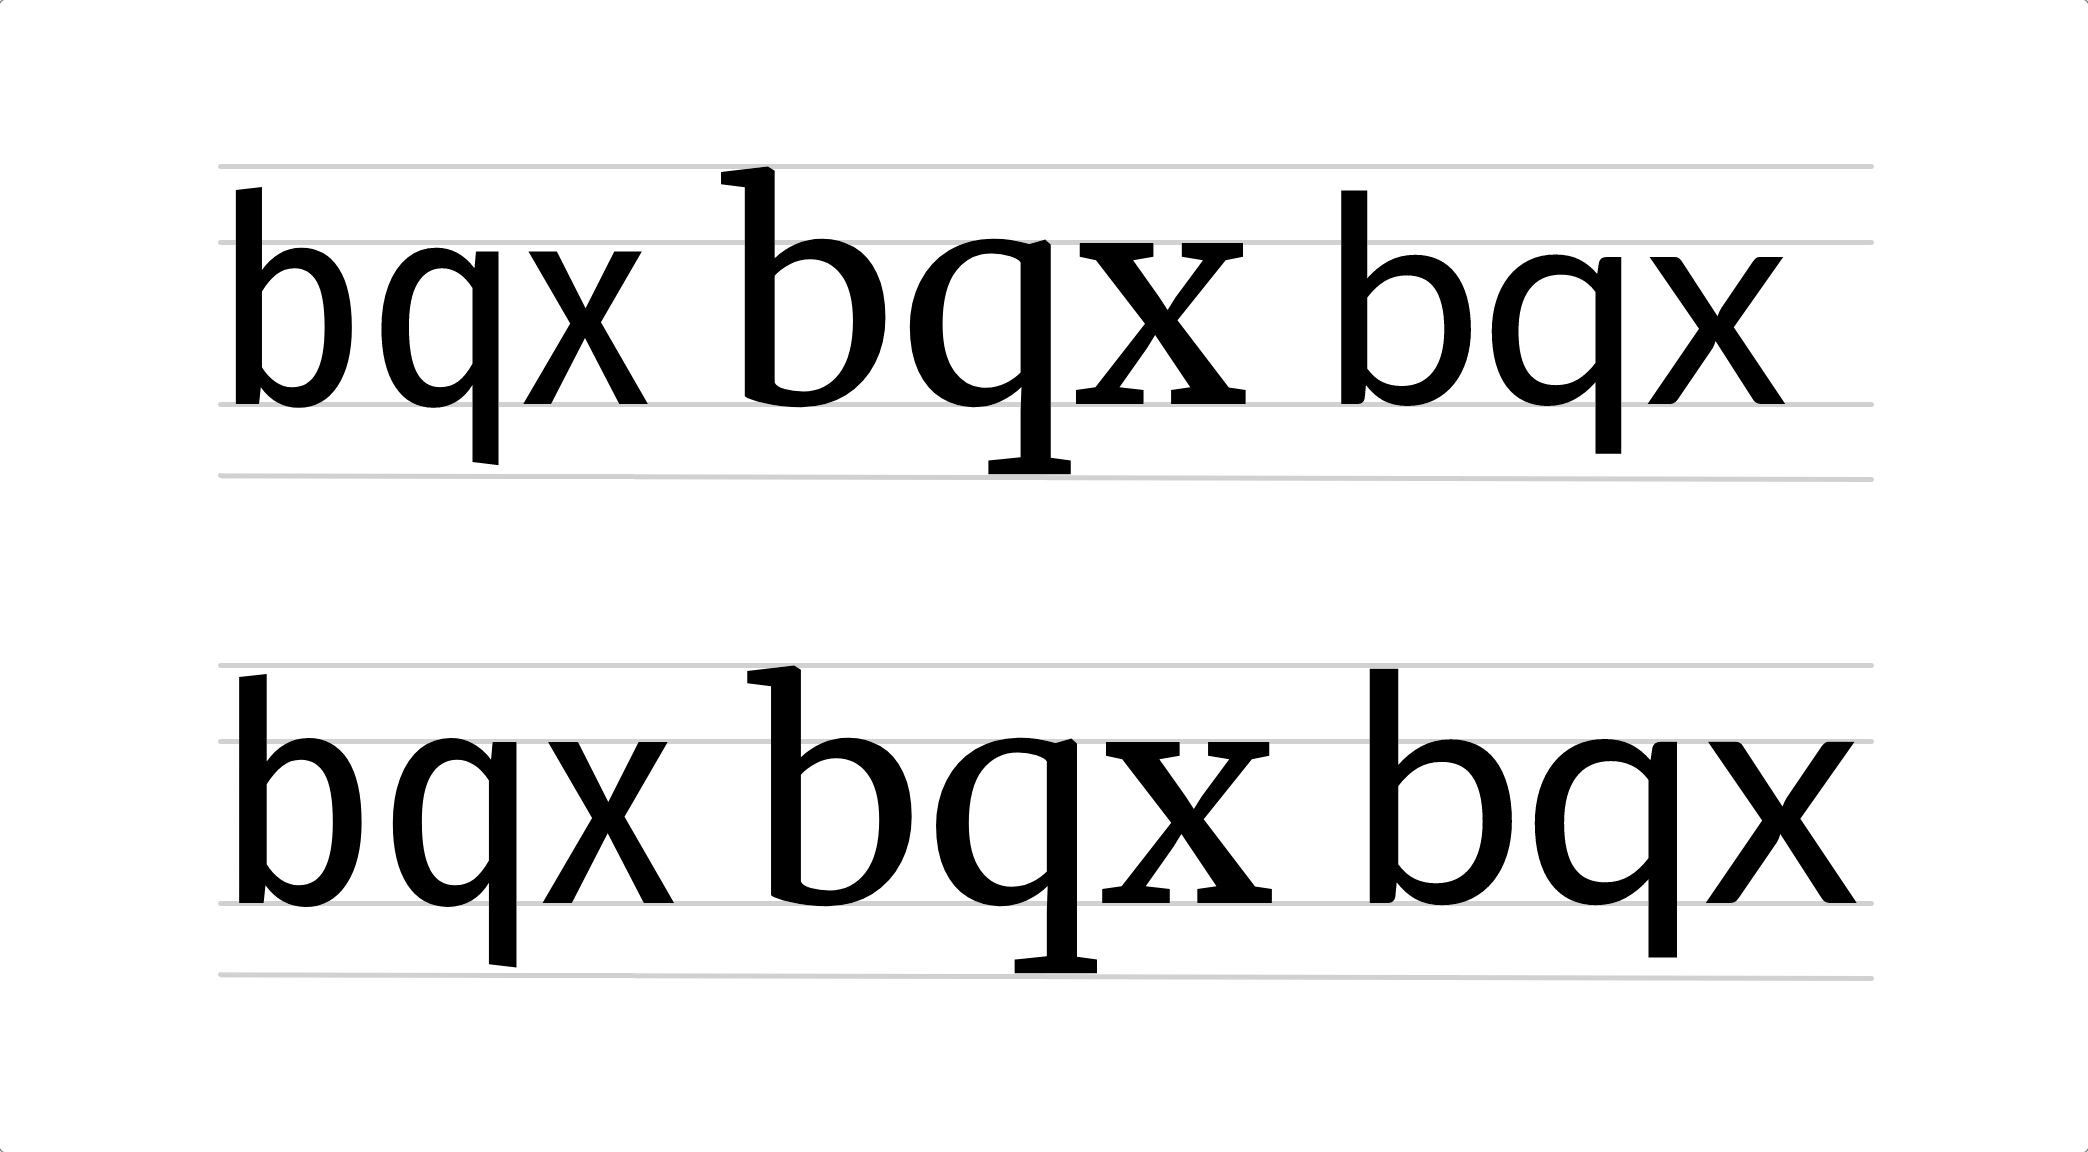
\includegraphics[width=\linewidth]{bvos}
  \caption{Comparison of body (top) versus optical (bottom) sizes on three typefaces: Fira Sans, Merriweather, and Lato. To match the optical size of Merriweather (center), Fira Sans (left) must be sized to 106\% of Merriweather's body size; Lato (right) to 110\%.} The top and bottom lines of each set represent the ascender and descender lines, respectively. The middle two lines illustrate the x-height.
  \Description{A screenshot showing different visual sizes on three different typefaces, and their visually uniform size when adjusted.}
  \label{fig:bvos}
\end{figure}


But rather than try different size values in an unstudied way, students can scaffold text-sizing according to common defaults and accessibility guidelines. By default, most desktop browsers set their base font-size to sixteen pixels. A good reset stylesheet should not interfere with that default size. The latest version of the Web Content Accessibility Guidelines (WCAG) refrains from making any specific text-size prescriptions; the WCAG does, however, note that “the smallest font size used on major browsers for unspecified text would be a reasonable size to assume for the font,” and also that “point size should be obtained from the user agent, or calculated based on font metrics as the user agent does” \cite{w3c:wcag}.

The Lighthouse Guild, formerly the National Association for Visually Handicapped, recommends a size range of 16 to 18 points, while noting the differences between typefaces\cite{lhg:mtl}. Although the ADA Standards are silent on text-sizing, the WCAG includes some suggested constraints for text sizing: Success Criteria 1.4.3 and 1.4.6 suggest a “large-scale” text size of 18 points for regular text and 14 points for bold text. Additionally, Success Criterion 1.4.4 calls for users to be able to resize text up to 200\% “without loss of content or functionality” \cite{w3c:wcag}, meaning that students can experiment with smaller sizes, provided that those sizes work when doubled: either by adjusting the value the stylesheet or using the zoom feature in their development browser.

In introducing those values to students, it’s necessary to explain to students the conversion from points to pixels. While the pixel once represented both a physical and a logical unit, the W3C distinguishes between the physical pixels on a screen and logical reference pixels \cite[§~5.2]{w3c:values}, which may involve lighting multiple physical pixels on high-density displays. Values expressed as pixels, \verb|px|, in CSS are always reference pixels. One point is 1/72 of an inch, while CSS pixels are approximated as 1/96 of an inch, making 1 point roughly 1.333 CSS pixels. The range from 14 to 18 points can be therefore be expressed as a CSS-pixel range of roughly 19 to 24 pixels.

\subsection{Establishing the Baseline Grid}

Typographic convention recommends setting a baseline grid of about 120\% of the base font size for body text. The proper baseline grid for a page is determined both by the size of the body text as well as the width of the column. The number of words on a line of text in a column is known as the {\itshape measure}; a readable measure on a single column of text is often between 45 and 75 characters, including spaces \cite[pp. 26–27]{rb:style}. Smaller measures can be set closer than larger measures, so long as the space is doing its primary job: aiding the eye's movement comfortably from the end of one line of text to the beginning of the next.

Pixel values for the \verb|line-height| that divide evenly into 2, 3, and 4 are convenient for  expressing half-, third-, and quarter-line adjustments between elements, especially for beginning students.

\subsection{Sizing Accent Type}

\begin{figure}
  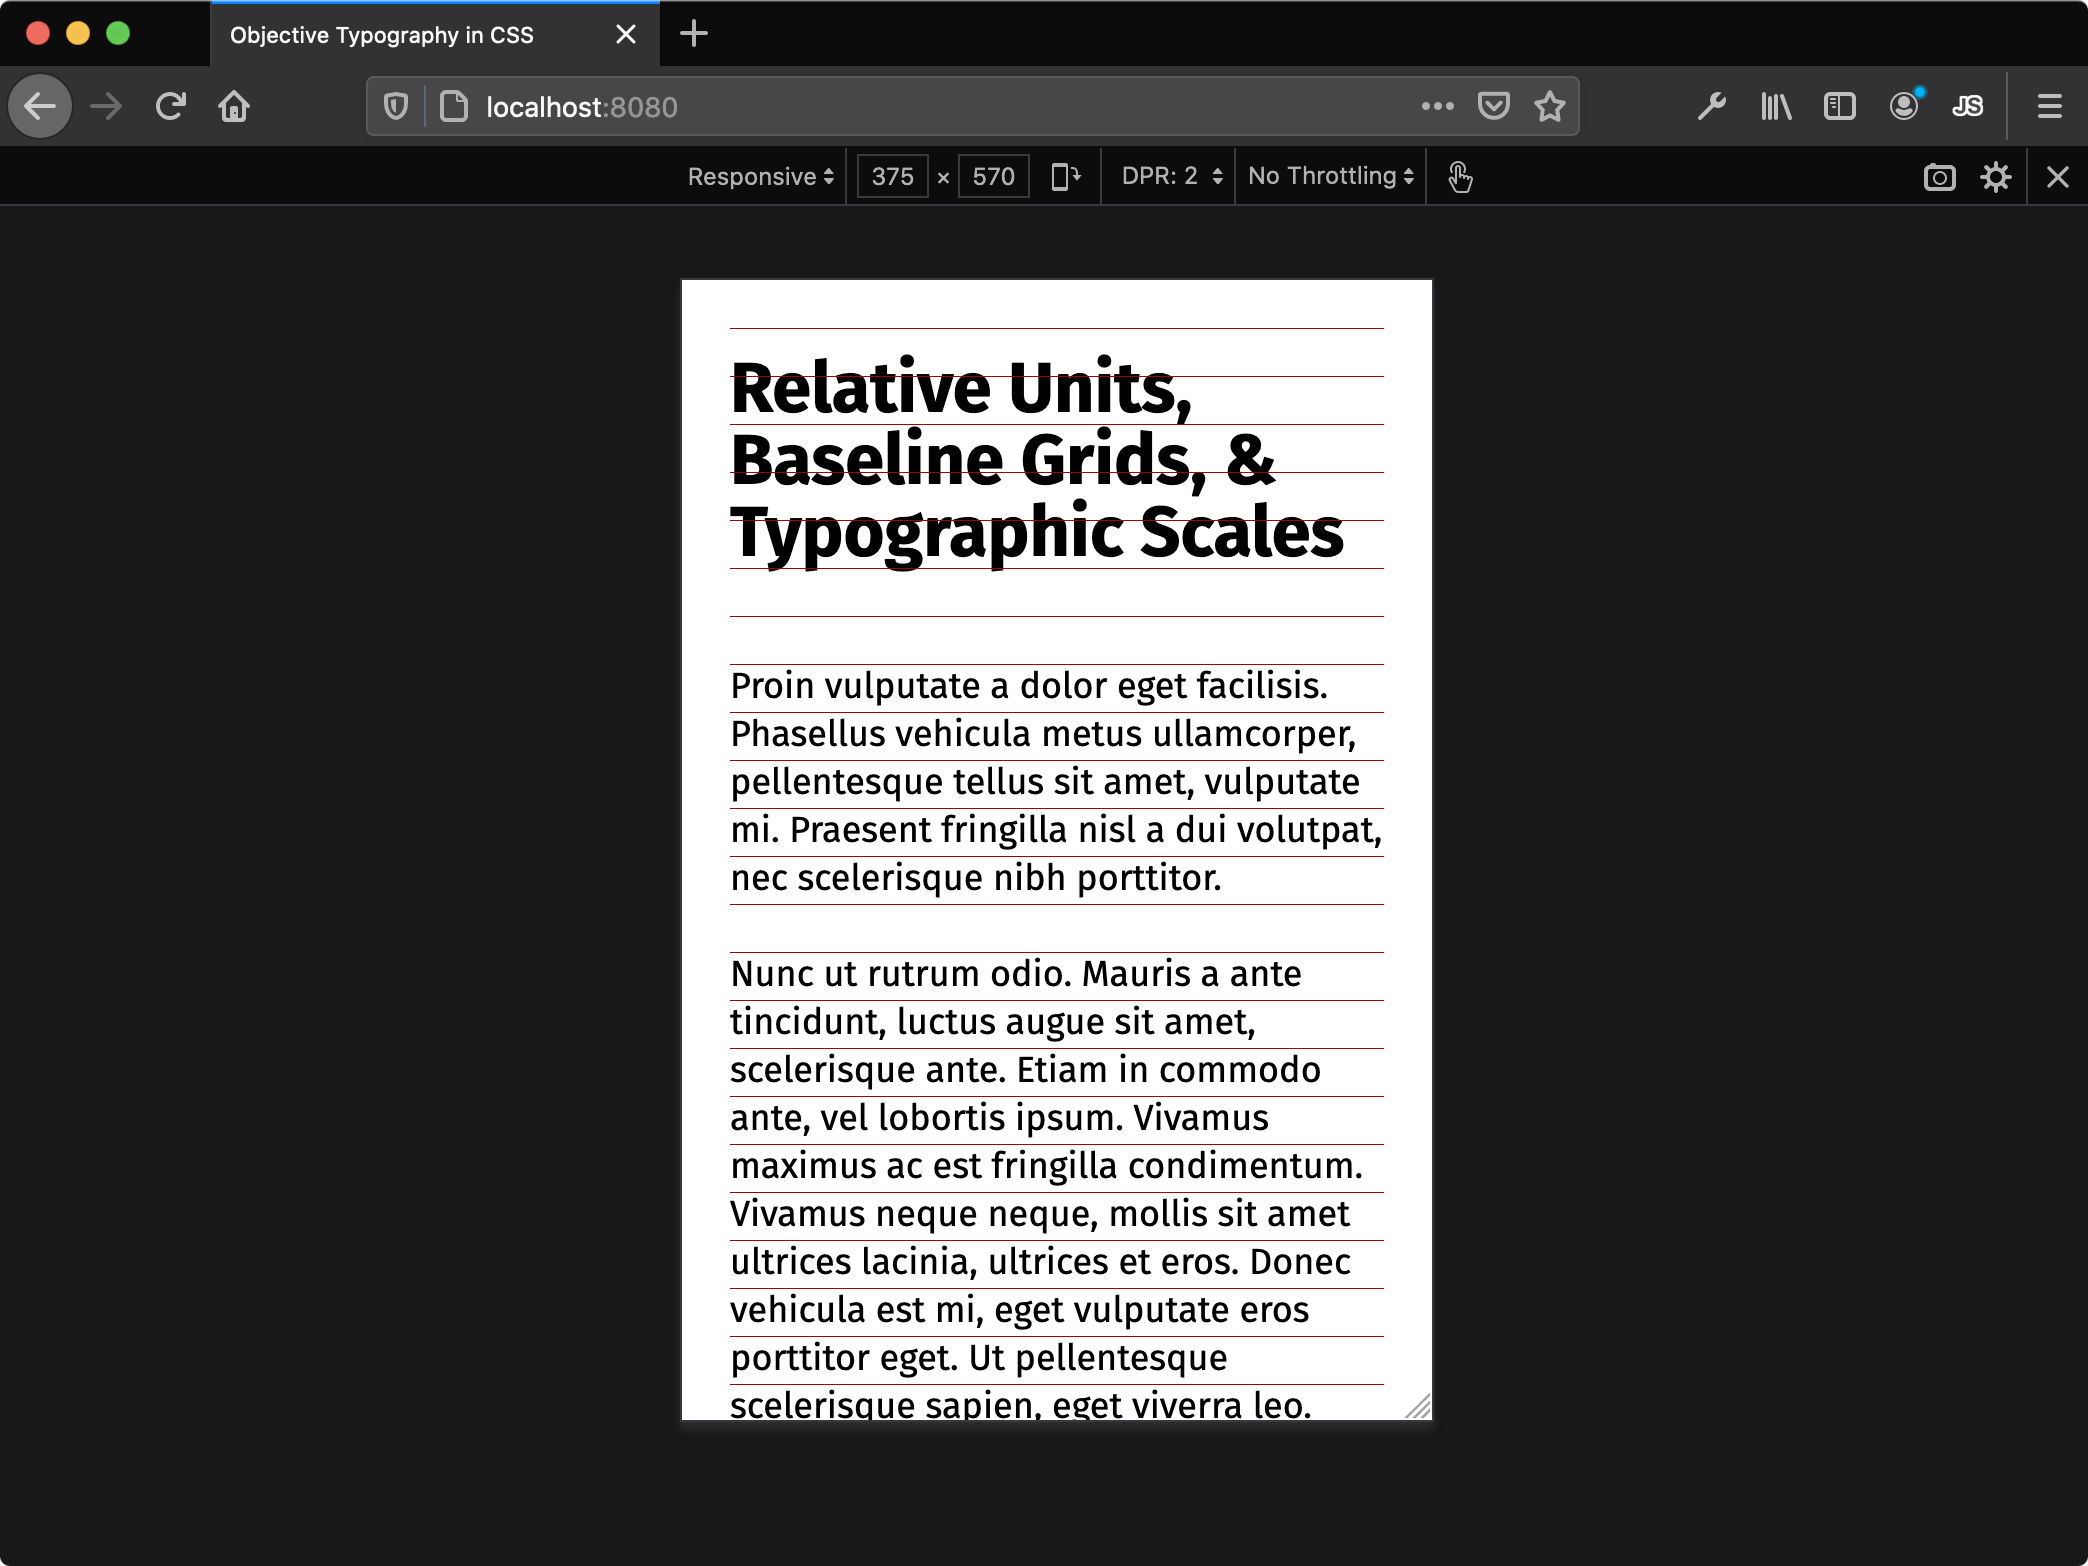
\includegraphics[width=\linewidth]{rdv-narrow}
  \caption{Text precisely set on a repeating baseline grid, with diagnostic grid lines shown.}
  \Description{The larger-sized headline copy occupies multiple grid lines, while each line of paragraph copy occupies just a single line.}
  \label{fig:rdv-narrow}
\end{figure}

The WCAG specification notes that “The 18 and 14 point sizes for roman texts are taken from the minimum size for large print (14pt) and the larger standard font size (18pt)” \cite{w3c:wcag}--“the larger standard font size” being derived, presumably, from the traditional typographers scale represented in the text-sizing drop-down menus of writing software (8, 9, 10, 11, 12, 14, 18, 24, 30, 36, 48, 60, 72, and 96 points).

Students should be encouraged to experiment with different mathematical ratios to determine a scale. A 4:3 ratio, for example, with a base font-size of 18px would include 10.13px, 13.503px, 18px, 23.994px, and so on.  To keep the base-line grid harmonious and functional, students need to adjust the \verb|line-height| property on text that is larger or substantially smaller than their base font-size, as shown in Figure \ref{fig:rdv-narrow}. Assuming a base font-size of 18px and a baseline grid of 22px, a heading set to 23.994px could be set comfortably on a gridline and a half (33px) or on a fully doubled gridline (44px).

\subsection{Refining the Grid}

Having established a base font size, a baseline grid, and a typographic scale, students move on to adding grid-determined space around elements. Both the \verb|margin| and \verb|padding| properties in CSS are appropriate for this task, although \verb|padding| behaves more predictably than \verb|margin|, as CSS will collapse adjacent margin values under particular circumstances.
An entire line of empty space can follow paragraph elements, as shown in Figure \ref{fig:rdv-narrow}, while list items can be separated by a half line of space. An additional half line of space set on the list itself ensures that a list will be followed by an entire line of empty space, just like paragraphs.
Additional space, derived from the \verb|line-height| value for the typographic grid, can be added to the \verb|html| selector on its \verb|padding| property.

\subsection{Relative Units and Responsiveness}

\begin{figure}
  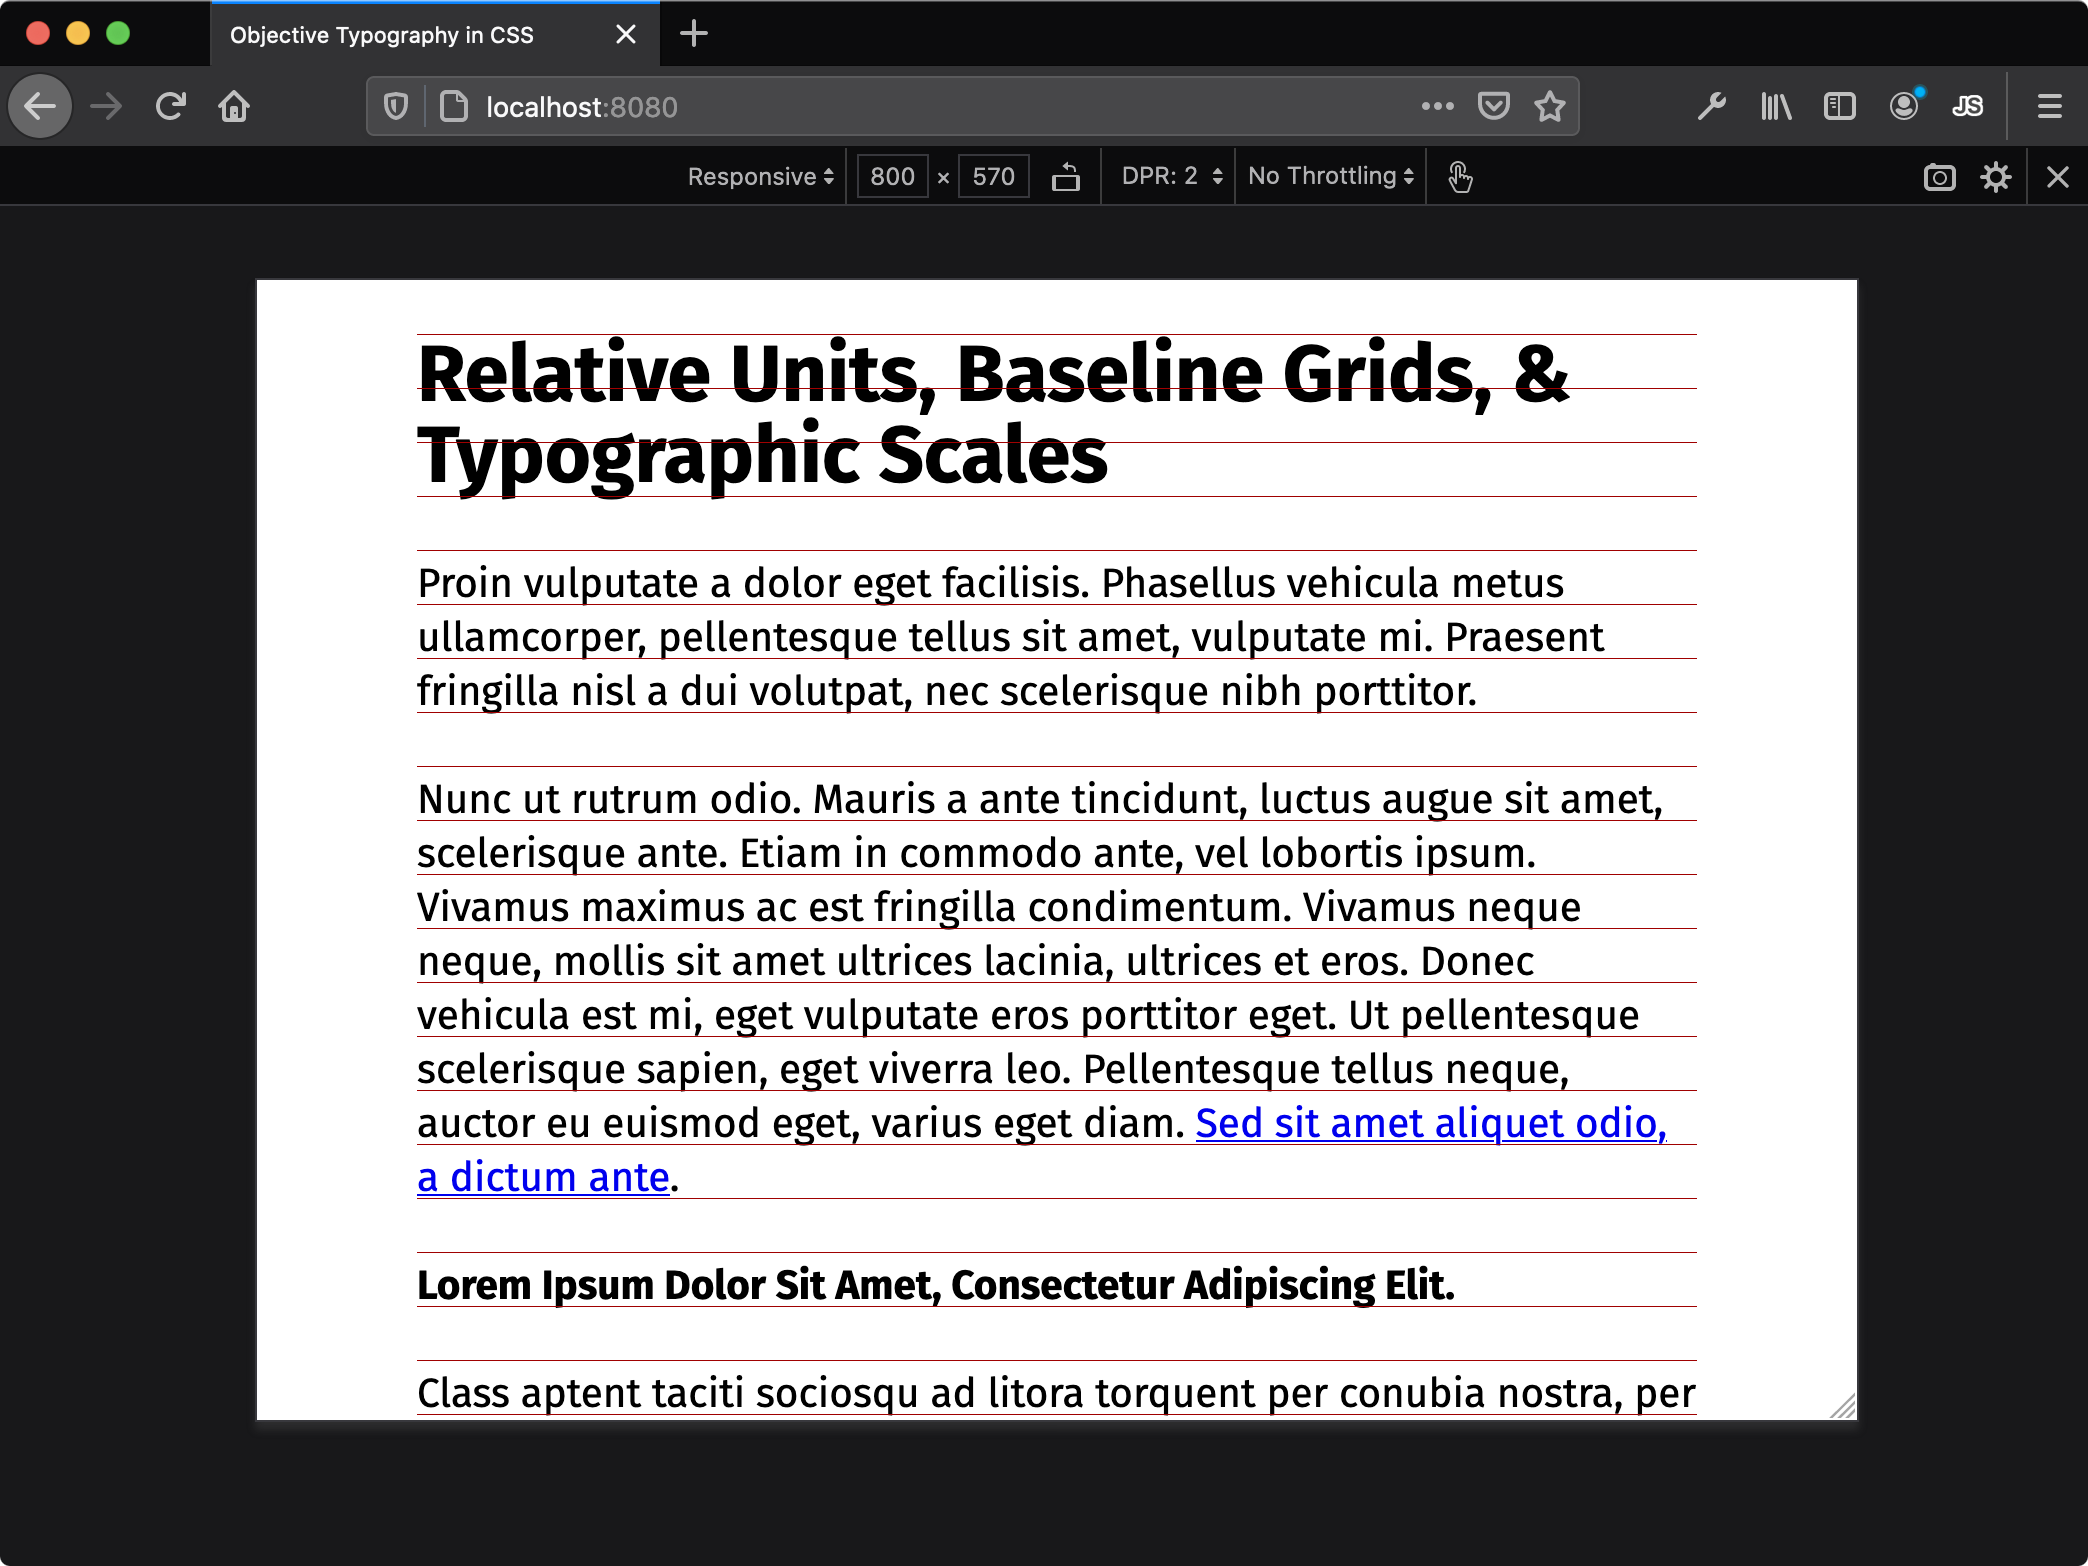
\includegraphics[width=\linewidth]{rdv-wide}
  \caption{Text set larger in a wider RDV viewport, with diagnostic grid lines shown.}
  \Description{At a larger viewport, the text is run larger. Gridlines are still constant, and size relationships between headings and boy copy remain. Additional space appears on either side of the single column of text.}
  \label{fig:rdv-wide}
\end{figure}

Having inspected their work, including with the aid of a grid overlay such as can be provided by Basehold.it or using a simple piece of instructor-provided SVG, students can confirm the accuracy of their baseline grid and their ability to size and set type to it. Students should then begin to gradually convert their absolute pixel-values to relative em-values. Because browsers default to a 16-pixel em, students can convert their base \verb|font-size| by dividing by 16. So a 19-pixel \verb|font-size| is equivalent to \verb|1.1875em|.

That value becomes the new em value for the page. If the 19-pixel text is set on a 24-pixel baseline, the relative \verb|line-height| value is arrived at by calculating 24/19, or \linebreak \verb|1.2631578947em|. With each conversion to a relative unit, students should refresh their  browsers and ensure their work still shows perfect alignment with the overlay . Any deviations from the grid means that a relative value was calculated incorrectly.

With relative units uniformly in place, students can then begin to open up the RDV viewport further. Once the lines of text become too long to comfortably read, or exceed the recommended lengths for line measures referenced earlier, and adjustment is needed.

The primary mechanism for making adjustments are via CSS media queries, which conditionally apply their contained CSS based on a screen condition, such as \verb|min-width|. Students should use the width as displayed in the RDV to write the query. A media query may need only to introduce a larger \verb|font-size| set on the \verb|html| selector. All of the carefully determined ratios and size relationships will scale accordingly. Additional space to the left and right sides of the text column can also help keep the measure of the lines readable, as in Figure \ref{fig:rdv-wide}.

\section{Conclusion}

This approach to CSS instruction has proved challenging but rewarding for students. Instead of focusing on a growing number of properties, students learn to take their time arriving at very precise values for a select number of properties. Anecdotally, since employing this method, students generally seem much more adept at commanding more complex CSS modules later in the course, particularly CSS Flexible Boxes and CSS Grid, both of which feature a large number of interdependent properties.

\subsection{Planned Enhancements}

During fall semester 2020, this approach will be enhanced further to include additional responsive typography features unique to CSS, including molten leading and CSS locks \cite{tb:ml,tb:cl}.

Simultaneously, so as to gather data about the effectiveness of the technique, an instrument will be developed and tested with volunteer enrolled students for further refinement in the future.

\bibliographystyle{ACM-Reference-Format}
\bibliography{stolley.bib}

\end{document}
